\documentclass[10pt]{report}
\usepackage[utf8]{inputenc}
\usepackage[italian]{babel}
\usepackage{multicol}
\usepackage[bookmarks]{hyperref}
\usepackage[a4paper, total={18cm, 25cm}]{geometry}
\usepackage{graphicx}
\usepackage{xcolor}
\usepackage{textcomp}
\graphicspath{ {./img/} }
\usepackage{listings}
\usepackage{makecell}
\lstdefinestyle{customasm}{
  belowcaptionskip=1\baselineskip,
  frame=line,
  xleftmargin=\parindent,
  language=[x86masm]Assembler,
  basicstyle=\ttfamily,
  commentstyle=\itshape\color{purple!40!black},
}
\lstset{escapechar=@,style=customasm}
\lstnewenvironment{C}
  {\lstset{language=C++,frame=none}}
  {}
\begin{document}
\title{Machine Learning}
\author{Federico Matteoni}
\date{A.A. 2021/22}
\renewcommand*\contentsname{Index}

\maketitle
\begin{multicols}{2}
\tableofcontents
\end{multicols}
\pagebreak
\section{Introduction}
What is ML? Area of research combining aims of creating computers that could learn and powerful and adaptive statistical tools with rigorous foundation in computational science. Luxury or necessity? Growing availability and need for analysis of empirical data and difficult to provide intelligence and adaptivity by programming it. Change of paradigm.\\
Examples: spam classification, written text recognition\ldots No or poor prior knowledge and rules for solving the problem, but easier to have a source of training experience.\\
ML is considered the latest general-purpose technology, capable of drastically affect pre-existing economic and social structures. And already has. The ultimate aim is to bring benefits to the people by solving big and small problems, accelerating human progress and empowering humans to add intelligence in any other science field.
\paragraph{Machine Learning} We restrict to the computational framework: principles, methods and algorithms for learning and prediction, from experience. Building a model to be used for predictions. Common framework: infer a model or a \textbf{function} from a set of examples which allows the generalization (accurate response to new data).\\
When can we use ML? Be aware of the opportunity and awareness. ML is useful when there's no or poor theory surrounding the phenomenon, or uncertain, noisy or incomplete data which hinders formalization of solutions. The requests are: source of training experience (representative data) and a tolerance on the precision of results. The best examples are models to solve real-world problems that are difficult to be treated with traditional techniques: face and voice recognition (knowledge too difficult to formalize in an algorithm), predicting biding strength of molecules to proteins (not enough human knowledge) and personalized behavior, such as recommendation systems, scoring messages according to user preferences\ldots
\paragraph{Definition} The ML studies and proposes methods to build functions/hypothesis from examples of observed data that fits the known examples and able to generalize, with reasonable accuracy, for new data (according to verifiable results and under statistical and computational conditions and criteria.
\paragraph{Data} Data \textbf{represents the available experience}. Representation problem: capturing the structure of the analyzed objects. Flat (attribute-value), structured\ldots, categorical or continuous, missing data\ldots \textbf{preprocessing}: variable scaling, encoding, selection\ldots
\paragraph{Task} The task defines the purpose of the application: knowledge that we want to achieve? which is the helpful nature of the result? what information are available?\\
\textbf{Predictive} task, classification and regression: function approximation\\
\textbf{Descriptive} task, cluster analysis and association rules: find subsets or groups of unclassified data.
\begin{center}
	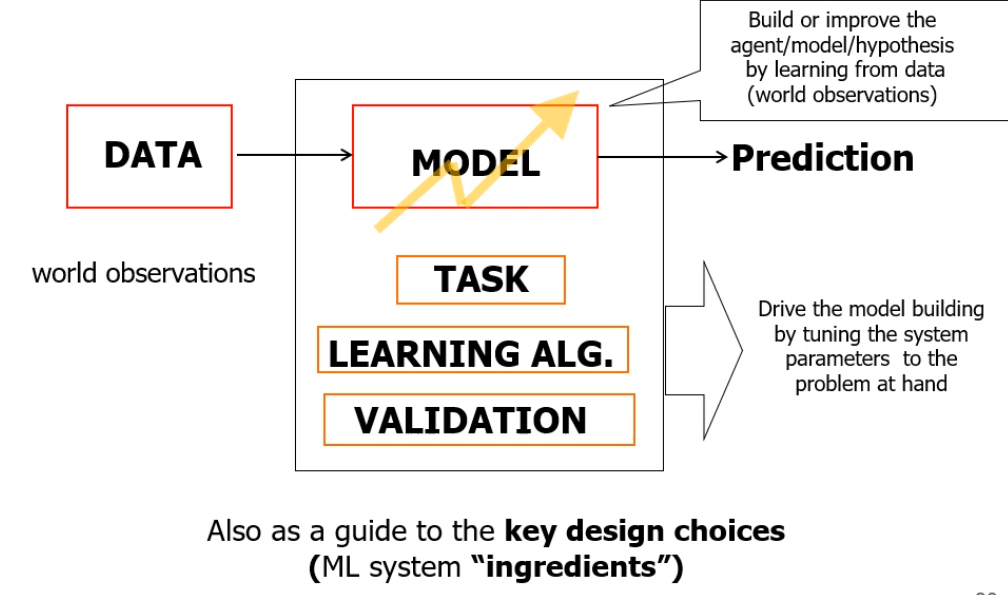
\includegraphics[scale=0.5]{1.png}
\end{center}
\pagebreak
\paragraph{Supervised learning} Given a set of training examples as $\langle$input, output$\rangle$ = $\langle x,d\rangle$ (\textbf{labeled examples}) for an unknown function $f$, find a \textit{good approximation} of $f$, an hypothesis $h$ that can be used for making predictions on unseen data $x'$.\\
The target $d$ can be:
\begin{list}{}{}
	\item Discrete value, for \textbf{classification tasks}.\\
	$f(x) \in \{1,2,\ldots,k\}$\\
	Patterns, feature vectors, are seen as members of a class and the goal is to assign the new patterns observed to the correct class (or label)\\
	If the number of possible classes is two, then $f$ is a \textit{boolean function} and the task is called \textbf{binary classification} or \textbf{concept learning}: true or false, positive or negative, 0 or 1\ldots\\
	If the number of classes is greater that two then is a \textbf{multi-class classification task}.
	\item Real continuous value, for \textbf{regression tasks}.\\
	The patterns are seen as sets of variables (real values), and the task is a curve fitting task. The process aims to estimate a real-value function based of a finite set of noisy samples $\langle x, f(x) +$ random noise$\rangle$
\end{list}
\paragraph{Unsupervised learning} No teacher. The training set is a set of unlabeled data $\langle x\rangle$. Examples: clustering, finding natural groupings in a set of data.
\paragraph{Learning algorithm} Basing on data, task and model: heuristic search through the hypothesis space $H$ of the \textbf{best hypothesis}. I. e. the best approximation of the unknown target function, typically searching for the $h$ with the minimum \textit{error}. $H$ may not coincide with the set of all possible function and the search cannot be exhaustive, we need to make \textbf{assumpitons} (\textbf{inductive bias}).
\paragraph{Learning} Also called:
\begin{list}{}{}
	\item Inference, in statistics
	\item Adapting, in biology and systems
	\item Optimizing, in mathematics
	\item Training, in neural networks
	\item Function approximations, in mathematics
	\item \ldots
\end{list}
After introducing data, task, model and learning algorithm we will focus on: inductive bias, loss and concepts of generalization and validation.
\paragraph{Inductive bias} To set up a model we can make assumptions about the nature of the target function, concerning either:
\begin{list}{}{}
	\item constraints in the model, \textbf{language bias} (in the hypothesis space $H$, due to the set of hypothesis that we can express or consider
	\item constraints or preferences in learning algorithm/search strategy, \textbf{search bias} which is preferred
	\item or both
\end{list}
Such assumptions are needed to obtain an useful model for the ML aims, i.e. a model with generalization capabilities.\\
We can imagine learning a discrete function with discrete inputs assuming \textbf{conjunctive rules}, so using a \textbf{language bias} to work with a restricted hypothesis space.
\paragraph{Version Space} An hypothesis $h$ is consistent with the TR if $h(x) = d(x)$ for each training example $\langle x, d(x)\rangle$.\\
The \textbf{version space} $VS_{H, TR}$ is the subset of $H$ of the hypothesis consistent with all the training examples $\langle x, d(x)\rangle$ in the TR.\\
It's possible to do an exhaustive search in an efficient way, using clever algorithms. This means finding the set of all the hypothesis $h$ consistent with the TR set. 
\paragraph{Unbiased Learner} The language bias (ex: using only conjunctive rules, may be too restrictive: if the target concept is not in $H$ it cannot be represented in $H$. We can use an $H$ that expresses every teachable concept (among propositions), that means that $H$ is the set of all possible subsets of $X$: the power set $P(X)$. If $n = 10$ binary inputs, then $|X| = 2^{10} = 1024$ and $|P(X)| = 2^{1024} = 10^{308}$ possible concepts, which is much more than the number of the atoms in the universe.\\
An unbiased learner is unable to generalize: the only examples that are unambiguously classified by an unbiased learner represented with the VS are the training examples themselves. Each unobserved instance will be classified positively by exactly half of the hypothesis in the VS and negative by the other half. Indeed: $\forall\: h$ consistent with $x_i$, $\exists\:h'$ identical to $h$ except $h'(x_i) \neq h(x_i)$, $h\in$ VS $\Rightarrow h'\in$ VS (because they are identical on the TR)\\\\
Why prefer the search bias? In ML we use flexible approaches (expressive hypothesis spaces with universal capability of the models, for example neural networks or decision trees. We avoid the language bias, so we do not exclude a priori the unknown target function, but we focus on the search bias (ruled by the learning algorithm).
\paragraph{Loss} How to measure the quality of an approximation? We want to measure the distance between $h(x)$ and $d$, using a loss function/measure $L(h(x), d)$ for a pattern $x$ which has high value in cases of bad approximation. The error (or risk or loss) is an expected value of this $L$, for example $E(w) = \frac{1}{l}\sum_{p=1}^l L(h(x_p), d_p)$. Different $L$ for different tasks. Examples of loss functions:
\begin{list}{}{}
	\item Regression: $L(h(x_p), d_p) = (d_p - h(x_p))^2$, the squared error. MSE (mean squared error) over the data set
	\item Classification: $L(h(x_p), d_p) = \left\{\begin{array}{l l}
		0 & h(x_p) = d_p\\
		1 & else
	\end{array}\right.$
\end{list}
\paragraph{Learning and generalization} Learning: search for a \textbf{good function} in a function space from known data (typically minimizing an error/loss). \textbf{Good} with respect to generalization error: it measures how accurately the model predicts over novel samples of data (\textbf{measured over \underline{new} data}).\\
Generalization is the crucial point of ML. Performance in ML is the generalization accuracy or \textit{predictive accuracy} estimated by the error on the test set.
\paragraph{ML issues} Inferring general functions from known data is an ill posed problem, which means that in general the solution is not unique because we can't expect the exact solution with finite data. What can we represent? And so, what can we learn?\\
Learning phase: building the model including training. The prediction phase is evaluating the learned function over new never-seen-before samples (generalization capability). Inductive learning hypothesis: any $h$ that approximates $f$ well on training examples will also approximate $f$ well on new unseen instances $x$.\\
\textbf{Overfitting}: a learner overfits data if it outputs an hypothesis $h\in H$ having true/generalization error (risk) $R$ and empirical (training) error $E$, but there's another $h'\in H$ with $E' > E$ and $R' < R$, which means that $h'$ is the better one despite having a worse fitting.
\paragraph{Statistical Learning Theory} Under what mathematical conditions is a model able to generalize? We want to investigate the generalization capability of a model, measured as a risk or test error, the role of the model complexity and the role of the number of data.\\
\textbf{Formal Setting}: approximate a function $f(x)$, with $d$ target ($d = f(x) +$ noise), minimizing the \textbf{risk function} $$R = \int L(d, h(x))\:dP(x,d)$$ which is the \textbf{true error over all the data}, given:
\begin{list}{}{}
	\item a value $d$ from the teacher and the probability distribution $P(x,d)$
	\item a loss function $L(h(x),d) = (d - h(x))^2$
\end{list}
We search for $h\in H\:|\: min\:R$, but we only have the finite data set $TR = (x_p, d_p)$ with $p = 1\ldots l$. Looking for $h$ means minimizing the empirical risk (the training error $E$), finding the best values for the model free parameters $$R_{emp} = \frac{1}{l}\sum_{p=1}^l (d_p - h(x_p))^2$$
The inductive principle is the \textbf{ERM}, Empirical Risk Minimization: can we use $R_{emp}$ to approximate $R$?
\paragraph{Vapnik-Chervoneniks dim and SLT} Given the VC dimension (simply VC), a measure of complexity of $H$ and by that we mean its flexibility to fit data.\\
The VC-bound states that it holds with probability $\frac{1}{\delta}$ that $$R \leq R_{emp} + \epsilon\left(\frac{1}{l}, \textsl{VC},\frac{1}{\delta}\right)$$
\begin{list}{}{}
	\item $\epsilon$ is a function called VC-confidence, that grows with VC and decreases with higher $l$ and $\delta$
	\item $R_{emp}$ decreases using complex models (with high VC)
	\item $\delta$ is the confidence, and it rules the probability that the bound holds.\\
	$\delta = 0.01 \Rightarrow$ the bound holds with probability $0.99$
\end{list}
Intuitively:
\begin{list}{}{}
	\item Higher $l$ (data) $\Rightarrow$ lower VC confidence and bound closer to $R$
	\item A too simple model, meaning with low VC, can be not sufficient due to high $R_{emp}$ (\textbf{underfitting})
	\item An higher VC with fix $l \Rightarrow$ lower $R_{emp}$ but VC and hence $R$ may increase (\textbf{overfitting})
\end{list}
\paragraph{Structural risk minimization} Minimize the bound! There are different bounds formulations according to different classes of $f$, of tasks\ldots\\
In other words, we can make a good approximation of $f$ from examples, provided that we have a good number of data and the complexity of the model is suitable for the task.
\paragraph{Complexity control} The Statistical Learning Theory allows for a formal framing of the problem of generalization and overfitting, providing an analytic upper bound to the risk $R$ for the prediction over all the data, regardless of the type of learning algorithm or the details of the model. So \textbf{the machine learning is well founded}, the learning risk can be analytically limited and only a few concepts are fundamental. This leads to new models (such as the Support Vector Machine) and other methods that directly consider the control of the complexity in the construction of the model.
\paragraph{Validation} Central role for the applications and the project. Two aims:
\begin{list}{}{}
	\item \textbf{Model Selection}: estimating the performance (\textbf{generalization error}) of different models in order to choose the best one. This includes searching for the best hyperparameters of the model.\\
	It returns a model.
	\item \textbf{Model Assessment}: with the final model, estimating/evaluating its prediction error/risk (\textbf{generalization error}) over new test data.\\
	It returns an estimation.
\end{list}
\textbf{Golden rule}: keep the two goals separated and use different datasets for each one.\\\\
In an ideal world, we'd have a large training set, a large validation set for model selection and a very large external unseen data test set. With finite and often small data sets we have just an estimation of the generalization performance. We have to use some techniques: hold-out and k-fold cross validation, for example.
\begin{list}{}{}
	\item \textbf{Hold-Out}: we partition the dataset $D$ into \textbf{training set} TR, \textbf{validation/selection set} VL and \textbf{test set} TS.\\
	All three are disjoint: TR is used to run the training algorithm, VL can be used to select the best model (hyperparameters tuning) and the \textbf{TS is only used for model assessment}.
	\begin{center}
		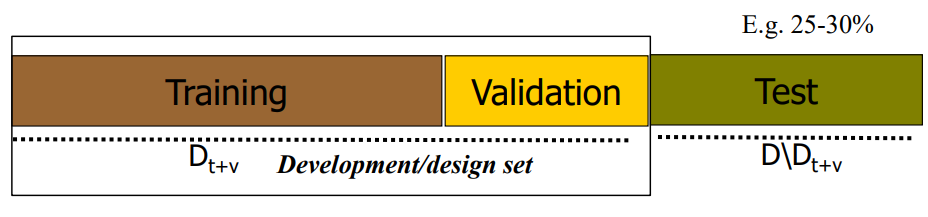
\includegraphics[scale=0.5]{2.png}
	\end{center}
	\item \begin{multicols}{2}
	\textbf{K-Fold}: this technique can make use of insufficient data. We split the dataset $D$ into $k$ mutually esclusive subsets $D_1,\ldots, D_k$, we train on $D - D_i$ and test it on $D_i$.\\
	This can be applied to both VL and TS splitting. Can be computationally very expensive and there's the issue of choosing the number of folds $k$.
	\begin{center}
		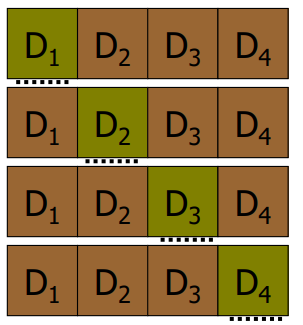
\includegraphics[scale=0.5]{3.png}
	\end{center}
	\end{multicols}
\end{list}
\paragraph{Classification accuracy} %TODO slide 154 di ML-21-INTRO-first-lectures-v0.11.pdf

% 24/09
\paragraph{} $E(w) = \Sum_{p=1}^l (y_p - x_p^T w)^2$\\
$\frac{\gradient E(w)}{\gradient W_j} = \ldots$ %TODO calc and first half of class
\paragraph{Gradient Descent: final discussion}
\paragraph{Linear models} Language bias: $H$ is a set of linear functions.\\Search Bias: ordered search guided by the least squares minimization goal. For instance, we could prefer a different method to obtain\ldots\\ %TODO
To extend: polynomial regression.
\end{document}